\documentclass[aspectratio=1610,onlymath]{beamer}
% \documentclass[aspectratio=1610,onlymath,handout]{beamer}

% Macros used by all lectures, but not necessarily by excercises

%%% General setup and dependencies:

% \usetheme[ddcfooter,nosectionnum]{tud}
\usetheme[nosectionnum,pagenum,noheader]{tud}
% \usetheme[nosectionnum,pagenum]{tud}

% Increase body font size to a sane level:
\let\origframetitle\frametitle
% \renewcommand{\frametitle}[1]{\origframetitle{#1}\normalsize}
\renewcommand{\frametitle}[1]{\origframetitle{#1}\fontsize{10pt}{13.2}\selectfont}
\setbeamerfont{itemize/enumerate subbody}{size=\small} % tud defaults to scriptsize!
\setbeamerfont{itemize/enumerate subsubbody}{size=\small}
% \setbeamerfont{normal text}{size=\small}
% \setbeamerfont{itemize body}{size=\small}

\renewcommand{\emph}[1]{\textbf{#1}}

\def\arraystretch{1.3}% Make tables even less cramped vertically

\usepackage[ngerman]{babel}
\usepackage[utf8]{inputenc}
\usepackage[T1]{fontenc}

%\usepackage{graphicx}
\usepackage[export]{adjustbox} % loads graphicx
\usepackage{import}
\usepackage{stmaryrd}
\usepackage[normalem]{ulem} % sout command
% \usepackage{times}
\usepackage{txfonts}

% \usepackage[perpage]{footmisc} % reset footnote counter on each page -- fails with beamer (footnotes gone)
\usepackage{perpage}  % reset footnote counter on each page
\MakePerPage{footnote}

\usepackage{tikz}
\usetikzlibrary{arrows,positioning}
% Inspired by http://www.texample.net/tikz/examples/hand-drawn-lines/
\usetikzlibrary{decorations.pathmorphing}
\pgfdeclaredecoration{penciline}{initial}{
    \state{initial}[width=+\pgfdecoratedinputsegmentremainingdistance,
    auto corner on length=1mm,]{
        \pgfpathcurveto%
        {% From
            \pgfqpoint{\pgfdecoratedinputsegmentremainingdistance}
                      {\pgfdecorationsegmentamplitude}
        }
        {%  Control 1
        \pgfmathrand
        \pgfpointadd{\pgfqpoint{\pgfdecoratedinputsegmentremainingdistance}{0pt}}
                    {\pgfqpoint{-\pgfdecorationsegmentaspect
                     \pgfdecoratedinputsegmentremainingdistance}%
                               {\pgfmathresult\pgfdecorationsegmentamplitude}
                    }
        }
        {%TO 
        \pgfpointadd{\pgfpointdecoratedinputsegmentlast}{\pgfpoint{1pt}{1pt}}
        }
    }
    \state{final}{}
}
\tikzset{handdrawn/.style={decorate,decoration=penciline}}
\tikzset{every shadow/.style={fill=none,shadow xshift=0pt,shadow yshift=0pt}}
% \tikzset{module/.append style={top color=\col,bottom color=\col}}

% Use to make Tikz attributes with Beamer overlays
% http://tex.stackexchange.com/a/6155
\tikzset{onslide/.code args={<#1>#2}{%
  \only<#1| handout:0>{\pgfkeysalso{#2}} 
}}
\tikzset{onslideprint/.code args={<#1>#2}{%
  \only<#1>{\pgfkeysalso{#2}} 
}}

%%% Title -- always set this first

\newcommand{\defineTitle}[3]{
	\newcommand{\lectureindex}{#1}
	\title{Formale Systeme}
	\subtitle{\href{\lectureurl}{#1. Vorlesung: #2}}
	\author{\href{http://korrekt.org/}{Markus Kr\"{o}tzsch}}
%	\author{\href{http://www.sebastian-rudolph.de}{Sebastian Rudolph} in Vertretung von \href{http://korrekt.org/}{Markus Kr\"{o}tzsch}}
	\date{#3}
	\datecity{TU Dresden}
% 	\institute{Computational Logic}
}

%%% Table of contents:

\RequirePackage{ifthen}

\newcommand{\highlight}[2]{%
	\ifthenelse{\equal{#1}{\lectureindex}}{\alert{#2}}{#2}%
}

\def\myspace{-0.7ex}
\newcommand{\printtoc}{
\begin{tabular}{r@{$\quad$}l}
\highlight{1}{1.} & \highlight{1}{Willkommen/Einleitung formale Sprachen}\\[\myspace]
\highlight{2}{2.} & \highlight{2}{Grammatiken und die Chomsky-Hierarchie}\\[\myspace]
\highlight{3}{3.} & \highlight{3}{Endliche Automaten}\\[\myspace]
\highlight{4}{4.} & \highlight{4}{Complexity of FO query answering}\\[\myspace]
\highlight{5}{5.} & \highlight{5}{Conjunctive queries}\\[\myspace]
\highlight{6}{6.} & \highlight{6}{Tree-like conjunctive queries}\\[\myspace]
\highlight{7}{7.} & \highlight{7}{Query optimisation}\\[\myspace]
\highlight{8}{8.} & \highlight{8}{Conjunctive Query Optimisation / First-Order~Expressiveness}\\[\myspace]
\highlight{9}{9.} & \highlight{9}{First-Order~Expressiveness / Introduction to Datalog}\\[\myspace]
\highlight{10}{10.} & \highlight{10}{Expressive Power and Complexity of Datalog}\\[\myspace]
\highlight{11}{11.} & \highlight{11}{Optimisation and Evaluation of Datalog}\\[\myspace]
\highlight{12}{12.} & \highlight{12}{Evaluation of Datalog (2)}\\[\myspace]
\highlight{13}{13.} & \highlight{13}{Graph Databases and Path Queries}\\[\myspace]
\highlight{14}{14.} & \highlight{14}{Outlook: database theory in practice}
\end{tabular}
}

\newcommand{\overviewslide}{%
\begin{frame}\frametitle{Overview}
\printtoc
\medskip

Siehe \href{\lectureurl}{course homepage [$\Rightarrow$ link]} for more information and materials
\end{frame}
}

%%% Colours:

\usepackage{xcolor,colortbl}
\definecolor{redhighlights}{HTML}{FFAA66}
\definecolor{lightblue}{HTML}{55AAFF}
\definecolor{lightred}{HTML}{FF5522}
\definecolor{lightpurple}{HTML}{DD77BB}
\definecolor{lightgreen}{HTML}{55FF55}
\definecolor{darkred}{HTML}{CC4411}
\definecolor{darkblue}{HTML}{176FC0}%{1133AA}
\definecolor{nightblue}{HTML}{2010A0}%{1133AA}
\definecolor{alert}{HTML}{176FC0}
\definecolor{darkgreen}{HTML}{36AB14}
\definecolor{strongyellow}{HTML}{FFE219}
\definecolor{devilscss}{HTML}{666666}

\newcommand{\redalert}[1]{\textcolor{darkred}{#1}}

%%% Style commands

\newcommand{\quoted}[1]{\texttt{"}{#1}\texttt{"}}
\newcommand{\squote}{\texttt{"}} % straight quote
\newcommand{\Sterm}[1]{\ensuremath{\mathtt{\textcolor{purple}{#1}}}}    % letters in alphabets
\newcommand{\Snterm}[1]{\textsf{\textcolor{darkblue}{#1}}} % nonterminal symbols
\newcommand{\Sntermsub}[2]{\Snterm{#1}_{\Snterm{#2}}} % nonterminal symbols
\newcommand{\Slang}[1]{\textbf{\textcolor{black}{#1}}}    % languages
\newcommand{\Slangsub}[2]{\Slang{#1}_{\Slang{#2}}}    % languages
% Code
\newcommand{\Scode}[1]{\textbf{#1}}    % reserved words in program listings, e.g., "if"
\newcommand{\Scodelit}[1]{\textcolor{purple}{#1}}    % literals in program listings, e.g., strings
\newcommand{\Scomment}[1]{\textcolor{gray}{#1}}    % comment in program listings

\newcommand{\epstrastar}{\mathrel{\mathord{\stackrel{\epsilon}{\to}}{}^*}} % transitive reflexive closure of epsilon transitions in an epslion-NFA

\newcommand{\narrowcentering}[1]{\mbox{}\hfill#1\hfill\mbox{}}

\newcommand{\defeq}{\mathrel{:=}}

\newcommand{\Smach}[1]{\ensuremath{\mathcal{#1}}}    % machines

%%% Slide layout commands:

\newcommand{\sectionSlide}[1]{
\frame{\begin{center}
\LARGE
#1
\end{center}}
}
\newcommand{\sectionSlideNoHandout}[1]{
\frame<handout:0>{\begin{center}
\LARGE
#1
\end{center}}
}

\newcommand{\mydualbox}[3]{%
 \begin{minipage}[t]{#1}
 \begin{beamerboxesrounded}[upper=block title,lower=block body,shadow=true]%
    {\centering\usebeamerfont*{block title}#2}%
    \raggedright%
    \usebeamerfont{block body}
%     \small
    #3%
  \end{beamerboxesrounded}
  \end{minipage}
}
% 
\newcommand{\myheaderbox}[2]{%
 \begin{minipage}[t]{#1}
 \begin{beamerboxesrounded}[upper=block title,lower=block title,shadow=true]%
    {\centering\usebeamerfont*{block title}\rule{0pt}{2.6ex} #2}%
  \end{beamerboxesrounded}
  \end{minipage}
}

\newcommand{\mycontentbox}[2]{%
 \begin{minipage}[t]{#1}%
 \begin{beamerboxesrounded}[upper=block body,lower=block body,shadow=true]%
    {\centering\usebeamerfont*{block body}\rule{0pt}{2.6ex}#2}%
  \end{beamerboxesrounded}
  \end{minipage}
}

\newcommand{\mylcontentbox}[2]{%
 \begin{minipage}[t]{#1}%
 \begin{beamerboxesrounded}[upper=block body,lower=block body,shadow=true]%
    {\flushleft\usebeamerfont*{block body}\rule{0pt}{2.6ex}#2}%
  \end{beamerboxesrounded}
  \end{minipage}
}

% label=180:{\rotatebox{90}{{\footnotesize\textcolor{darkgreen}{Beispiel}}}}
% \hspace{-8mm}\ghost{\raisebox{-7mm}{\rotatebox{90}{{\footnotesize\textcolor{darkgreen}{Beispiel}}}}}\hspace{8mm}
\newcommand{\examplebox}[1]{%
	\begin{tikzpicture}[decoration=penciline, decorate]
		\pgfmathsetseed{1235}
		\node (n1) [decorate,draw=darkgreen, fill=darkgreen!10,thick,align=left,text width=\linewidth, inner ysep=2mm, inner xsep=2mm] at (0,0) {#1};
% 		\node (n2) [align=left,text width=\linewidth,inner sep=0mm] at (n1.92) {{\footnotesize\raisebox{3mm}{\textcolor{darkgreen}{Beispiel}}}};
% 		\node (n2) [decorate,draw=darkgreen, fill=darkgreen!10,thick, align=left,text width=\linewidth,inner sep=2mm] at (n1.90) {{\footnotesize\raisebox{0mm}{\textcolor{darkgreen}{Beispiel}}}};
	\end{tikzpicture}%
}%

\newcommand{\codebox}[1]{%
	\begin{tikzpicture}[decoration=penciline, decorate]
		\pgfmathsetseed{1236}
		\node (n1) [decorate,draw=strongyellow, fill=strongyellow!10,thick,align=left,text width=\linewidth, inner ysep=2mm, inner xsep=2mm] at (0,0) {#1};
	\end{tikzpicture}%
}%

\newcommand{\defbox}[1]{%
	\begin{tikzpicture}[decoration=penciline, decorate]
		\pgfmathsetseed{1237}
		\node (n1) [decorate,draw=darkred, fill=darkred!10,thick,align=left,text width=\linewidth, inner ysep=2mm, inner xsep=2mm] at (0,0) {#1};
	\end{tikzpicture}%
}%

\newcommand{\theobox}[1]{%
	\begin{tikzpicture}[decoration=penciline, decorate]
		\pgfmathsetseed{1240}
		\node (n1) [decorate,draw=darkblue, fill=darkblue!10,thick,align=left,text width=\linewidth, inner ysep=2mm, inner xsep=2mm] at (0,0) {#1};
	\end{tikzpicture}%
}%

\newcommand{\anybox}[2]{%
	\begin{tikzpicture}[decoration=penciline, decorate]
		\pgfmathsetseed{1240}
		\node (n1) [decorate,draw=#1, fill=#1!10,thick,align=left,text width=\linewidth, inner ysep=2mm, inner xsep=2mm] at (0,0) {#2};
	\end{tikzpicture}%
}%


\newsavebox{\mybox}%
\newcommand{\doodlebox}[2]{%
\sbox{\mybox}{#2}%
	\begin{tikzpicture}[decoration=penciline, decorate]
		\pgfmathsetseed{1238}
		\node (n1) [decorate,draw=#1, fill=#1!10,thick,align=left,inner sep=1mm] at (0,0) {\usebox{\mybox}};
	\end{tikzpicture}%
}%

% Common notation

\usepackage{amsmath,amssymb,amsfonts}
\usepackage{xspace}

\newcommand{\lectureurl}{https://iccl.inf.tu-dresden.de/web/FS2016}

\DeclareMathAlphabet{\mathsc}{OT1}{cmr}{m}{sc} % Let's have \mathsc since the slide style has no working \textsc

% Dual of "phantom": make a text that is visible but intangible
\newcommand{\ghost}[1]{\raisebox{0pt}[0pt][0pt]{\makebox[0pt][l]{#1}}}

\newcommand{\tuple}[1]{\langle{#1}\rangle}

%%% Annotation %%%

\usepackage{color}
\newcommand{\todo}[1]{{\tiny\color{red}\textbf{TODO: #1}}}



%%% Old macros below; move when needed

\newcommand{\blank}{\text{\textvisiblespace}} % empty tape cell for TM

% table syntax
\newcommand{\dom}{\textbf{dom}}
\newcommand{\adom}{\textbf{adom}}
\newcommand{\dbconst}[1]{\texttt{"#1"}}
\newcommand{\pred}[1]{\textsf{#1}}
\newcommand{\foquery}[2]{#2[#1]}
\newcommand{\ground}[1]{\textsf{ground}(#1)}
% \newcommand{\foquery}[2]{\{#1\mid #2\}} %% Notation as used in Alice Book
% \newcommand{\foquery}[2]{\tuple{#1\mid #2}}

\newcommand{\quantor}{\mathord{\reflectbox{$\text{\sf{Q}}$}}} % the generic quantor

% logic syntax
\newcommand{\Inter}{\mathcal{I}} %used to denote an interpretation
\newcommand{\Jnter}{\mathcal{J}} %used to denote another interpretation
\newcommand{\Knter}{\mathcal{K}} %used to denote yet another interpretation
\newcommand{\Zuweisung}{\mathcal{Z}} %used to denote a variable assignment

% query languages
\newcommand{\qlang}[1]{{\sf #1}} % Font for query languages
\newcommand{\qmaps}[1]{\textbf{QM}({\sf #1})} % Set of query mappings for a query language

%%% Complexities %%%

\hyphenation{Exp-Time} % prevent "Ex-PTime" (see, e.g. Tobies'01, Glimm'07 ;-)
\hyphenation{NExp-Time} % better that than something else

% \newcommand{\complclass}[1]{{\sc #1}\xspace} % font for complexity classes
\newcommand{\complclass}[1]{\ensuremath{\mathsc{#1}}\xspace} % font for complexity classes

\newcommand{\ACzero}{\complclass{AC$_0$}}
\newcommand{\LogSpace}{\complclass{L}}
\newcommand{\NLogSpace}{\complclass{NL}}
\newcommand{\PTime}{\complclass{P}}
\newcommand{\NP}{\complclass{NP}}
\newcommand{\coNP}{\complclass{coNP}}
\newcommand{\PH}{\complclass{PH}}
\newcommand{\PSpace}{\complclass{PSpace}}
\newcommand{\NPSpace}{\complclass{NPSpace}}
\newcommand{\ExpTime}{\complclass{ExpTime}}
\newcommand{\NExpTime}{\complclass{NExpTime}}
\newcommand{\ExpSpace}{\complclass{ExpSpace}}
\newcommand{\TwoExpTime}{\complclass{2ExpTime}}
\newcommand{\NTwoExpTime}{\complclass{N2ExpTime}}
\newcommand{\ThreeExpTime}{\complclass{3ExpTime}}
\newcommand{\kExpTime}[1]{\complclass{#1ExpTime}}
\newcommand{\kExpSpace}[1]{\complclass{#1ExpSpace}}


\defineTitle{2}{Grammatiken und die Chomsky-Hierarchie}{1. November 2020}

\begin{document}

\maketitle

\sectionSlideNoHandout{Rückblick}

\begin{frame}\frametitle{Wiederholung}

\begin{itemize}
\item Formale Sprachen sind in Praxis und Theorie sehr wichtig
\item Ein \redalert{Alphabet} ist eine nichtleere, endliche Menge von Symbolen
\item Ein \redalert{Wort} ist eine endliche Sequenz von Symbolen
\item Eine \redalert{Sprache} ist eine Menge von Wörtern
\item Es gibt viele \redalert{Operationen auf Sprachen} ($\cap, \cup, \overline{\phantom{L}}, \circ, {}^*, {}^+, \setminus$)
\item Man kann Sprachen auf viele Arten beschreiben\\
(von denen wir noch einige genauer kennen lernen werden)
\end{itemize}

\end{frame}

\sectionSlide{Sprachen beschreiben}

\begin{frame}\frametitle{Wie kann man Sprachen beschreiben?}

Die Operationen aus der vorigen Vorlesung können das schon ganz gut:
\medskip

\examplebox{Beispiel (Wiederholung):
Die Menge aller gültigen Schreibweisen für Dezimalzahlen kann wie folgt definiert werden:\\[1.5ex]

\narrowcentering{$ \Slang{Dezimalzahl} =  \Big(\{\epsilon\}\cup \{\Sterm{+},\Sterm{-}\}\Big) \circ \Big(\{\Sterm{0}\}\cup (\Slang{Z}\setminus\{\Sterm{0}\})\circ\Slang{Z}^*\Big) \circ \Big( \{\epsilon\}\cup \{\Sterm{.}\}\Slang{Z}^+ \Big) $}\\[1.5ex]

mit $\Slang{Z}=\{\Sterm{0},\Sterm{1},\Sterm{2},\Sterm{3},\Sterm{4},\Sterm{5},\Sterm{6},\Sterm{7},\Sterm{8},\Sterm{9}\}$.
}
\bigskip

Wir haben hier eine unendliche Sprache mit einfachen Grundoperationen aus endlichen Sprachen konstruiert.
\bigskip

\redalert{Funktioniert das für alle Sprachen?}

\end{frame}

\begin{frame}\frametitle{Wie viele Wörter gibt es?}

\pause

\theobox{Satz: Es gibt \redalert{abzählbar viele} Wörter über jedem Alphabet $\Sigma$. Jede Sprache ist also entweder endlich oder abzählbar unendlich.}
\pause

\emph{Idee:} Zum "`Abzählen"' reihen wir die Wörter in $\Sigma^*$ der Länge nach auf, beginnend mit den kurzen Wörtern.\\
Zum Beispiel: $\epsilon, \Sterm{a}, \Sterm{b}, \Sterm{aa}, \Sterm{ab}, \Sterm{ba}, \Sterm{bb}, \Sterm{aaa}, \Sterm{aab},\ldots$
\smallskip
\pause

\emph{Beweis} (die gleiche Idee, aber etwas formaler):\\
\begin{itemize}
\item Laut Definition ist $\Sigma^* = \Sigma^0 \cup \Sigma^1 \cup \Sigma^2 \cup \ldots = \bigcup_{i\geq 0} \Sigma^i$.\\
\item Jede der Mengen $\Sigma^i$ ist endlich (es gibt nur endlich viele Wörter der Länge $i$).\\
\item Es gibt abzählbar viele Mengen $\Sigma^i$ (eine für jede natürliche \ghost{Zahl)}.\\
\item Eine abzählbare Vereinigung endlicher Mengen ist abzählbar.\\
\item Also ist $\Sigma^*$ abzählbar.\qed
\end{itemize}


\end{frame}

\begin{frame}\frametitle{Wie viele Sprachen gibt es?}

\pause

\theobox{Satz: Es gibt \redalert{überabzählbar viele} Sprachen über jedem beliebigen Alphabet $\Sigma$.}
\pause

\emph{Beweis:}
\begin{itemize}
\item Die Menge aller Wörter \alert{$\Sigma^*$ ist abzählbar unendlich}, selbst wenn $\Sigma$ nur ein Symbol enthält.
\item Eine Sprache ist eine beliebige Teilmenge von $\Sigma^*$.
\item Die Menge aller Sprachen über $\Sigma$ ist die Menge aller Teilmengen (\alert{Potenzmenge}) von $\Sigma^*$.
\item Die Kardinalität der Potenzmenge ist immer größer als die der Menge selbst (\alert{Satz von Cantor}).
\item Also gibt es überabzählbar viele Sprachen.\qed
\end{itemize}

\end{frame}

\begin{frame}\frametitle{Aus Kardinalitäten lernen}

\emph{Zusammenfassung:} Über jedem beliebigen Alphabet $\Sigma$ gibt es
\begin{itemize}
\item \redalert{abzählbar} viele Wörter
\item \redalert{überabzählbar} viele Sprachen
\end{itemize}
\bigskip\pause

\emph{Beobachtung:} Wir beschreiben Sprachen mit "`Wörtern"':
\begin{itemize}
\item Natürlichsprachliche Texte sind Wörter
\item Computerprogramme sind Wörter
\item Mathematische Formeln sind Wörter
\end{itemize}
Es gibt \redalert{viel mehr} Sprachen als Texte, Programme oder \ghost{Formeln!}
\pause
\bigskip

\theobox{Satz: Fast alle Sprachen können in keiner Weise endlich beschrieben werden.
Fast alle Sprachen werden durch kein Computerprogramm korrekt erkannt.}

Ein starker Satz, aber er gibt uns keine Hinweise, welche Sprachen man wie beschreiben kann.
Zum Beispiel gibt es eindeutig beschreibbare Sprachen, für die es kein Computerprogramm gibt.

\end{frame}

% Beispiele mit "Aussagen", die man beweisen kann

% Identitaeten ("Rechenregeln")

\sectionSlide{Grammatiken}

\begin{frame}\frametitle{Sprachen mit Grammatiken beschreiben}

Grammatiken sind die wichtigste Methode zur Beschreibung von Sprachen.
\bigskip

Sie verwenden \redalert{Ersetzungsregeln} um Wörter zu \redalert{erzeugen}.

\examplebox{Beispiel: Die folgende Grammatik erzeugt Dezimalzahlen.
\begin{align*}
\Snterm{Dezimalzahl} &\to \Snterm{Vorzeichen}\;\Snterm{DZahl} \mid \Snterm{DZahl}& (1)\\
\Snterm{Vorzeichen} &\to \Sterm{+} \mid \Sterm{-}& (2)\\
\Snterm{DZahl} &\to \Snterm{NatZahl} \mid \Snterm{NatZahl}\;\Sterm{.}\;\Snterm{Ziffernreihe}& (3)\\
\Snterm{NatZahl} &\to \Snterm{Ziffer} \mid \Snterm{ZifferAb1}\;\Snterm{Ziffernreihe}& (4)\\
\Snterm{Ziffernreihe} &\to \Snterm{Ziffer} \mid\Snterm{Ziffer}\;\Snterm{Ziffernreihe}& (5)\\
\Snterm{ZifferAb1} &\to \Sterm{1} \mid \Sterm{2} \mid \ldots \mid \Sterm{9}& (6)\\
\Snterm{Ziffer} &\to \Sterm{0} \mid \Sterm{1} \mid \Sterm{2} \mid \ldots \mid \Sterm{9}& (7)
\end{align*}

}

\end{frame}

\begin{frame}\frametitle{Grammatiken anwenden}

\scalebox{0.8}{
\examplebox{\vspace{-3ex}
\begin{align*}
\Snterm{Dezimalzahl} &\to \Snterm{Vorzeichen}\;\Snterm{DZahl} \mid \Snterm{DZahl}& (1)\\
\Snterm{Vorzeichen} &\to \Sterm{+} \mid \Sterm{-}& (2)\\
\Snterm{DZahl} &\to \Snterm{NatZahl} \mid \Snterm{NatZahl}\;\Sterm{.}\;\Snterm{Ziffernreihe}& (3)\\
\Snterm{NatZahl} &\to \Snterm{Ziffer} \mid \Snterm{ZifferAb1}\;\Snterm{Ziffernreihe}& (4)\\
\Snterm{Ziffernreihe} &\to \Snterm{Ziffer} \mid\Snterm{Ziffer}\;\Snterm{Ziffernreihe}& (5)\\
\Snterm{ZifferAb1} &\to \Sterm{1} \mid \Sterm{2} \mid \ldots \mid \Sterm{9}& (6)\\
\Snterm{Ziffer} &\to \Sterm{0} \mid \Sterm{1} \mid \Sterm{2} \mid \ldots \mid \Sterm{9}& (7)
\end{align*}
}}

Wir können folgende Ersetzungsschritte ausführen:
\[\begin{array}{@{}r@{}l@{}}
\Snterm{Dezimalzahl} & \pause\stackrel{(1)}{\Rightarrow} \Snterm{Vorzeichen}\;\Snterm{DZahl}
		\pause\stackrel{(2)}{\Rightarrow} \Sterm{-}\Snterm{DZahl}
		\pause\stackrel{(3)}{\Rightarrow} \Sterm{-}\Snterm{NatZahl}\Sterm{.}\Snterm{Ziffernreihe}\\
	& \pause\stackrel{(4)}{\Rightarrow} \Sterm{-}\Snterm{Ziffer}\Sterm{.}\Snterm{Ziffernreihe}
% 		\pause\stackrel{(7)}{\Rightarrow} \Sterm{-}\Snterm{ZifferAb1}\Sterm{.}\Snterm{Ziffernreihe}\\
		\pause\stackrel{(7)}{\Rightarrow} \Sterm{-}\Sterm{3}\Sterm{.}\Snterm{Ziffernreihe}\\
	& \pause\stackrel{(5)}{\Rightarrow} \Sterm{-}\Sterm{3}\Sterm{.}\Snterm{Ziffer}\;\Snterm{Ziffernreihe}
		\pause\stackrel{(5)}{\Rightarrow} \Sterm{-}\Sterm{3}\Sterm{.}\Snterm{Ziffer}\;\Snterm{Ziffer}\\
	&	\pause\stackrel{(7)}{\Rightarrow} \Sterm{-}\Sterm{3}\Sterm{.}\Sterm{1}\;\Snterm{Ziffer} \stackrel{(7)}{\Rightarrow} \Sterm{-}\Sterm{3}\Sterm{.}\Sterm{1}\Sterm{4}\\
\end{array}\]

\end{frame}

\begin{frame}\frametitle{Definition: Grammatik}

\defbox{
Eine \redalert{Grammatik} $G$ ist ein 4-Tupel $G=\tuple{V,\Sigma,P,S}$ bestehend aus:
\begin{itemize}
\item $V$ eine Menge von \redalert{Variablennamen}
\item $\Sigma$ ein Alphabet, disjunkt zu $V$ (d.h., $\Sigma\cap V=\emptyset$)
\item $P$ eine Menge von \redalert{Produktionsregeln} der Form $w\to v$ für beliebige Wörter $w$ und $v$ über $\Sigma\cup V$, wobei $w$ mindestens eine Variable enthält (d.h. $w,v\in(\Sigma\cup V)^*$ und $w\notin\Sigma^*$)
\item $S$ eine \redalert{Startvariable} aus $V$ (d.h. $S\in V$)
\end{itemize}
Die Elemente von $\Sigma$ nennt man auch \redalert{Terminalsymbole}, die Elemente von $V$ analog \redalert{Nicht-Terminalsymbole}.
}

Die zuvor verwendete Schreibweise $w\to v_1\mid v_2 \mid \ldots \mid v_n$ ist eine Abkürzung für die Produktionsregeln
$w\to v_1, w\to v_2,\ldots, w\to v_n$.

\end{frame}

\begin{frame}\frametitle{Beispiele: Grammatiken}

\examplebox{Beispiel: Eine Grammatik $\tuple{V,\Sigma,P,\Snterm{Start}}$ sei gegeben durch
$V=\{\Snterm{Start},\Snterm{Summe},\Snterm{Var}\}$,
$\Sigma=\{\Sterm{(},\Sterm{)},\Sterm{+},\Sterm{*},\Sterm{x},\Sterm{y},\Sterm{z}\}$ 
und Regeln $P$:\\[0.5ex]
\narrowcentering{$
\begin{array}{r@{}l}
\Snterm{Start} &{}\to \Snterm{Summe} \mid \Snterm{Summe}\;\Sterm{*}\;\Snterm{Start}\\
\Snterm{Summe} &{}\to \Sterm{(}\;\Snterm{Var}\;\Sterm{+}\;\Snterm{Var}\;\Sterm{)}\\
\Snterm{Var} &{}\to \Sterm{x} \mid \Sterm{y} \mid \Sterm{z}.
\end{array}
$}\\[0.5ex]
Diese Grammatik erzeugt zum Beispiel das Wort $\Sterm{(x+y)*(x+z)}$.%:
% 
% \begin{align*}
% \Snterm{Start} &\Rightarrow \Snterm{Summe}\;\Sterm{*}\;\Snterm{Start}
% 		\Rightarrow \Snterm{Summe}\;\Sterm{*}\;\Snterm{Summe}\\
% 	& \Rightarrow \Sterm{(}\Snterm{Var}\Sterm{+}\Snterm{Var}\Sterm{)}\;\Sterm{*}\;\Snterm{Summe}
% 		\Rightarrow \Sterm{(x+}\Snterm{Var}\Sterm{)}\;\Sterm{*}\;\Snterm{Summe}\\
% 	& \Rightarrow \Sterm{(x+y)}\;\Sterm{*}\;\Snterm{Summe}
% 		\Rightarrow \Sterm{(x+y)}\;\Sterm{*}\;\Sterm{(}\Snterm{Var}\Sterm{+}\Snterm{Var}\Sterm{)}\\
% 	& \Rightarrow \Sterm{(x+y)}\;\Sterm{*}\;\Sterm{(x+}\Snterm{Var}\Sterm{)}
% 		\Rightarrow \Sterm{(x+y)}\;\Sterm{*}\;\Sterm{(x+z)}
% \end{align*}
}\pause

\examplebox{Beispiel: Die selbe Sprache wird auch durch die Grammatik
$\tuple{\{\Snterm{Start},\Snterm{Var}\},\Sigma,P',\Snterm{Start}}$ definiert, mit $\Sigma$ wie oben und Regeln $P'$:\\[0.5ex]
\narrowcentering{$
\begin{array}{r@{}l}
\Snterm{Start} &{}\to \Sterm{(\Snterm{Var}+\Snterm{Var})}\\
\Sterm{(\Snterm{Var}+\Snterm{Var})} &{}\to \Sterm{(\Snterm{Var}+\Snterm{Var})*(\Snterm{Var}+\Snterm{Var})}\\
\Snterm{Var} &{}\to \Sterm{x}\mid\Sterm{y}\mid \Sterm{z}.
\end{array}
$}\\[0.5ex]
Es ist also erlaubt (1) Terminalsymbole durch Regeln zu verändern und (2) mehr als ein Symbol auf einmal zu
ersetzen. 
}

\end{frame}

\begin{frame}\frametitle{Beispiele: Diskussion}

Die Beispiele werfen \alert{wichtige Fragen} auf:
\begin{itemize}
\item Wie kann man herausfinden, ob zwei unterschiedliche Grammatiken die selbe Sprache beschreiben?
\item Muss man Grammatiken so allgemein definieren oder genügen auch vereinfachte Formen?
\item Kann man Grammatiken (automatisch) vereinfachen, ohne die Sprache zu verändern?
\end{itemize}

Antworten in dieser Vorlesung \ldots\bigskip

Erst einmal sollten wir die \alert{"`Sprache einer Grammatik"'} ordentlich definieren.

\end{frame}

\begin{frame}\frametitle{Definition: Ableitung}

\defbox{Sei $\tuple{V,\Sigma,P,S}$ eine Grammatik.
Die \redalert{1-Schritt-Ableitungsrelation} ist eine binäre Relation \redalert{$\Rightarrow$}
zwischen Wörtern aus $(V\cup\Sigma)^*$, so dass $u \Rightarrow v$ genau dann wenn:\\[1ex]
%
\narrowcentering{$u=w_1\, x\, w_2 \text{ und } v=w_1\, y\, w_2 \text{ und es gibt eine Regel }x\to y\in P$}\\[1ex]
%
wobei $w_1,w_2,x,y\in (V\cup\Sigma)^*$ beliebige Wörter sind.}

\medskip

\defbox{%
Die \redalert{Ableitungsrelation $\Rightarrow^*$} ist der reflexive, transitive Abschluss von
$\Rightarrow$, das heißt $u \Rightarrow^* v$ genau dann wenn:\\[1ex]
%
\narrowcentering{$u=w_1\Rightarrow w_2\Rightarrow \ldots\Rightarrow w_{n-1}\Rightarrow w_n=v$}\\[1ex]
% \narrowcentering{$u=w_1$ und $w_1\Rightarrow w_2$ und $\cdots{}$ und $w_{n-1}\Rightarrow w_n$ und $w_n=v$}\\[1ex]
%
wobei $n\geq 1$ und $w_1,\ldots,w_n\in (V\cup\Sigma)^*$ beliebige Wörter sind.
% \narrowcentering{es gibt Wörter $w_1,\ldots,w_n\in (V\cup\Sigma)^*$ für $n\geq 1$, so dass}\\\narrowcentering{$u=w_1$, $v=w_n$ und $w_1\Rightarrow w_2\Rightarrow \ldots\Rightarrow w_n$}\\[1ex]
%
Insbesondere gilt $u\Rightarrow^* u$ für alle $u\in (V\cup\Sigma)^*$ (Fall $n=1$).
}

{\footnotesize \textcolor{devilscss}{Anmerkung: Der Begriff "`Herleitungsrelation"' ist auch gebräuchlich. Wir verwenden "`Ableitung"' und "`Herleitung"' synonym.\\
Anmerkung 2: Manche Autoren schreiben $\vdash$ statt $\Rightarrow$.}}

\end{frame}

\begin{frame}\frametitle{Definition: Sprache einer Grammatik}

\defbox{Die \redalert{von einer Grammatik $G=\tuple{V,\Sigma,P,S}$ erzeugte Sprache $\textbf{L}(G)$} besteht aus allen Wörtern über $\Sigma$, die
man von $S$ ableiten kann:\\[1ex]
\narrowcentering{$\Slang{L}(G) = \{ w\in\Sigma^* \mid S\Rightarrow^* w \}$}
}\pause

\emph{Vereinfachung:} Für einfache Beispiele nehmen wir ab jetzt an, dass alle Großbuchstaben Variablen und
alle Kleinbuchstaben Terminalsymbole sind, wobei $\Snterm{S}$ die Startvariable ist.
\medskip

\examplebox{ Beispiel: Wir betrachten die Grammatik $G_{\text{id}}$ mit den Regeln:\\[1ex]
\narrowcentering{$\Snterm{S} \to \Snterm{B}\Snterm{A}\qquad\quad
	\Snterm{A} \to \Snterm{B}\Snterm{A} \mid \Snterm{Z}\Snterm{A} \mid \epsilon\qquad\quad
	\Snterm{B} \to \Sterm{b}\qquad\quad
	\Snterm{Z} \to \Sterm{z}
$}\\[0.5ex]
(Vereinfachte Version der "`Bezeichner"', wobei alle Buchstaben als $\Sterm{b}$ und alle Ziffern als $\Sterm{z}$ abgekürzt werden.)\medskip

Dann gilt $\Slang{L}(G_{\text{id}}) = \{\Sterm{b}\}\circ \{\Sterm{b},\Sterm{z}\}^*$.
}

\end{frame}

\begin{frame}\frametitle{Beweis zum Beispiel (1)}

\anybox{gray}{%
Für die Grammatik $G_{\text{id}}$ mit den Regeln\\[1ex]
\narrowcentering{$\Snterm{S} \to \Snterm{B}\Snterm{A}\qquad\quad
	\Snterm{A} \to \Snterm{B}\Snterm{A} \mid \Snterm{Z}\Snterm{A} \mid \epsilon\qquad\quad
	\Snterm{B} \to \Sterm{b}\qquad\quad
	\Snterm{Z} \to \Sterm{z}
$}\\[0.5ex]
gilt $\Slang{L}(G_{\text{id}}) = \{\Sterm{b}\}\circ \{\Sterm{b},\Sterm{z}\}^*$?\\
Das müsste man erst einmal beweisen \ldots
}\pause
\bigskip

\emph{Beweis:} Wir zeigen die beiden Richtungen\\ (1) $\Slang{L}(G_{\text{id}}) \subseteq \{\Sterm{b}\}\circ \{\Sterm{b},\Sterm{z}\}^*$ und (2) $\Slang{L}(G_{\text{id}}) \supseteq \{\Sterm{b}\}\circ \{\Sterm{b},\Sterm{z}\}^*$ getrennt.
\bigskip\pause

(1) Die Behauptung ist: "`jedes Wort in $\Slang{L}(G_{\text{id}})$ ist in $\{\Sterm{b}\}\circ \{\Sterm{b},\Sterm{z}\}^*$."'
\begin{itemize}
\item $\Slang{L}(G_{\text{id}})\subseteq \{\Sterm{b},\Sterm{z}\}^*$, weil $\{\Sterm{b},\Sterm{z}\}$ das Alphabet von $G_{\text{id}}$ ist
\item jedes Wort in $\Slang{L}(G_{\text{id}})$ beginnt mit $\Sterm{b}$, weil $\Snterm{S}$ nur durch $\Snterm{B}\Snterm{A}$ ersetzt werden kann und $\Snterm{B}$ nur durch $\Sterm{b}$
\item also ist $\Slang{L}(G_{\text{id}}) \subseteq \{\Sterm{b}\}\circ \{\Sterm{b},\Sterm{z}\}^*$
\end{itemize}

\end{frame}

\begin{frame}\frametitle{Beweis zum Beispiel (2)}

\anybox{gray}{%
\narrowcentering{$\Snterm{S} \to \Snterm{B}\Snterm{A}\qquad\quad
	\Snterm{A} \to \Snterm{B}\Snterm{A} \mid \Snterm{Z}\Snterm{A} \mid \epsilon\qquad\quad
	\Snterm{B} \to \Sterm{b}\qquad\quad
	\Snterm{Z} \to \Sterm{z}
$}
}%
\bigskip

\emph{Beweis (Fortsetzung):} Es fehlt noch die Rückrichtung.
% Wir zeigen die beiden Richtungen\\ (1) $\Slang{L}(G_{\text{id}}) \subseteq \{\Sterm{b}\}\circ \{\Sterm{b},\Sterm{z}\}^*$ und (2) $\Slang{L}(G_{\text{id}}) \supseteq \{\Sterm{b}\}\circ \{\Sterm{b},\Sterm{z}\}^*$ getrennt.
\bigskip

(2) Die Behauptung ist: "`jedes Wort in $\{\Sterm{b}\}\circ \{\Sterm{b},\Sterm{z}\}^*$ ist in $\Slang{L}(G_{\text{id}})$."'
\begin{itemize}
\item Sei $\Sterm{b}s_1 \ldots s_n$ mit $n\geq 0$ ein beliebiges Wort in $\{\Sterm{b}\}\circ \{\Sterm{b},\Sterm{z}\}^*$\\ (also $s_1,\ldots,s_n\in \{\Sterm{b},\Sterm{z}\}$)
\item Wir zeigen $\Sterm{b}s_1 \ldots s_n\in \Slang{L}(G_{\text{id}})$ indem wir eine Ableitung \ghost{angeben,}\\
d.h. wir zeigen $\Snterm{S} \Rightarrow^* \Sterm{b}s_1 \ldots s_n$
\item Die Ableitung beginnt immer so: $\Snterm{S} \Rightarrow \Snterm{B}\Snterm{A} \Rightarrow \Sterm{b}\Snterm{A}$
\item Jetzt müssen wir nur noch $\Snterm{A}\Rightarrow^* s_1 \ldots s_n$ zeigen. 
\end{itemize}

\end{frame}


\begin{frame}\frametitle{Beweis zum Beispiel (3)}

\anybox{gray}{%
\narrowcentering{$\Snterm{S} \to \Snterm{B}\Snterm{A}\qquad\quad
	\Snterm{A} \to \Snterm{B}\Snterm{A} \mid \Snterm{Z}\Snterm{A} \mid \epsilon\qquad\quad
	\Snterm{B} \to \Sterm{b}\qquad\quad
	\Snterm{Z} \to \Sterm{z}
$}
}%
\bigskip

\emph{Beweis (Fortsetzung):} Wir behaupten $\Snterm{A}\Rightarrow^* s_1 \ldots s_n$ für beliebige $n\geq 0$ und $s_1,\ldots,s_n\in \{\Sterm{b},\Sterm{z}\}$.
Die Ableitung ist in jedem konkreten Fall leicht gefunden, zum Beispiel für
$n=2$ und $s_1s_2=\Sterm{z}\Sterm{b}$ ergibt sich
$\Snterm{A}\Rightarrow \Snterm{Z}\Snterm{A}\Rightarrow\Sterm{z}\Snterm{A}\Rightarrow \Sterm{z}\Snterm{B}\Snterm{A}
\Rightarrow \Sterm{z}\Sterm{b}\Snterm{A}\Rightarrow \Sterm{z}\Sterm{b}$.
\bigskip\pause

Aber es gibt unendlich viele Fälle!\\\pause
$\leadsto$ Wir zeigen, wie man die Ableitung rekursiv konstruieren \ghost{kann.}\pause
% \bigskip
% 
\begin{itemize}
\item Für $n=0$ ist $s_1 \ldots s_n=\epsilon$ und $\Snterm{A}\Rightarrow\epsilon$ gilt direkt\pause
\item Für $n>0$ und $s_1=\Sterm{b}$ verwenden wir $\Snterm{A}\Rightarrow \Snterm{B}\Snterm{A}\Rightarrow\Sterm{b}\Snterm{A}$ und von da ab (rekursiv) die Ableitung
$\Snterm{A}\Rightarrow^* s_2 \ldots s_n$.\pause
\item Für $n>0$ und $s_1=\Sterm{z}$ verwenden wir $\Snterm{A}\Rightarrow \Snterm{Z}\Snterm{A}\Rightarrow\Sterm{z}\Snterm{A}$ und von\\da ab (rekursiv) die Ableitung
$\Snterm{A}\Rightarrow^* s_2 \ldots s_n$.\pause
\end{itemize}
Die Rekursion terminiert, da wir mit jedem Rekursionschritt kürzere Wörter ableiten.

\end{frame}

\begin{frame}\frametitle{Beweis zum Beispiel (4)}

\anybox{gray}{%
\narrowcentering{$\Snterm{S} \to \Snterm{B}\Snterm{A}\qquad\quad
	\Snterm{A} \to \Snterm{B}\Snterm{A} \mid \Snterm{Z}\Snterm{A} \mid \epsilon\qquad\quad
	\Snterm{B} \to \Sterm{b}\qquad\quad
	\Snterm{Z} \to \Sterm{z}
$}
}%
\bigskip

\emph{Beweis (Fortsetzung):} Der "`rekursiv konstruierte Beweis"' ist natürlich eine \redalert{vollständige Induktion}:
\medskip

\alert{Induktionsbehauptung:} $A\Rightarrow^* s_1\ldots s_n$ für alle $n\geq 0$ und \ghost{$s_1,\ldots,s_n\in \{\Sterm{b},\Sterm{z}\}$}\\
\alert{Induktionsanfang:} für $n=0$ gilt $A\Rightarrow^* \epsilon$\\
\alert{Induktionshypothese:} $A\Rightarrow^* s_1\ldots s_n$ gilt für $n$ und alle \ghost{$s_1,\ldots,s_n\in \{\Sterm{b},\Sterm{z}\}$}\\
\alert{Induktionschritt:} $A\Rightarrow^* s_1\ldots s_{n+1}$ gilt für alle $s_1,\ldots,s_n\in \{\Sterm{b},\Sterm{z}\}$, weil:\\
\begin{itemize}
\item wenn $s_1=\Sterm{b}$ dann $\Snterm{A}\Rightarrow \Snterm{B}\Snterm{A}\Rightarrow\Sterm{b}\Snterm{A}$
\item wenn $s_1=\Sterm{z}$ dann $\Snterm{A}\Rightarrow \Snterm{Z}\Snterm{A}\Rightarrow\Sterm{z}\Snterm{A}$
\item Behauptung folgt, da $\Snterm{A}\Rightarrow^* s_2\ldots s_{n+1}$ (Induktionshypothese)
\end{itemize}
\medskip\pause

\emph{Zusammenfassung Beweis Teil (2):}\\
Für beliebige Wörter $w$ gilt: wenn $w\in\{\Sterm{b}\}\circ \{\Sterm{b},\Sterm{z}\}^*$ dann $w\in\Slang{L}(G_{\text{id}})$.\\
Anders gesagt: $\{\Sterm{b}\}\circ \{\Sterm{b},\Sterm{z}\}^*\subseteq \Slang{L}(G_{\text{id}})$.
% Somit haben wir die Gesamtaussage (mehrfach) bewiesen.
\qed

\end{frame}


% Grammatik: Beispiel mit Ableitung,
% Produktionssystem, Ableitungsregel, (Nicht)Terminal, Start am Beispiel
% formale Definition
%	TODO: Notation Regeln: "->" oder "::=" oder was ganz anderes?
% Herleitungsrelation, Ableitung, erzeugte Sprache
% Beispielgrammatiken und ihre Sprachen (mit Beweis)

\sectionSlide{Die Chomsky-Hierarchie}

\begin{frame}\frametitle{Sprachen einteilen nach Grammatiken}

Die meisten Sprachen können \alert{nicht} mit Grammatiken beschrieben werden
{\footnotesize (abzählbar viele Grammatiken vs.\ überabzählbar viele Sprachen)}
\bigskip

\begin{itemize}
\item Die meisten \alert{praktisch relevanten} Sprachen haben aber eine Grammatik
\item Manche Sprachen kann man sogar mit einfacheren \alert{Sonderformen von Grammatiken} beschreiben
\end{itemize}
\bigskip

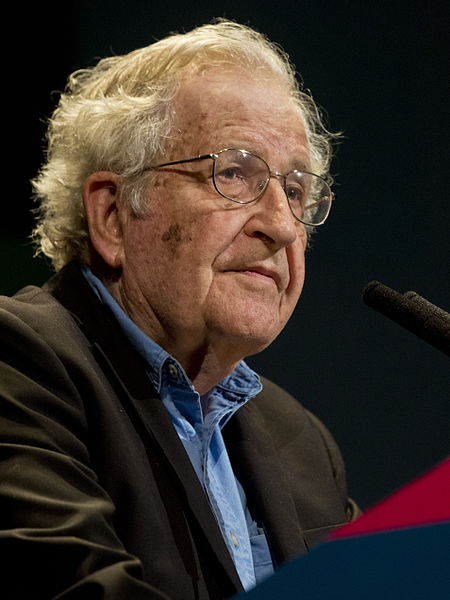
\includegraphics[width=3cm]{images/Noam-Chomsky-2015}
$\;$\rotatebox{90}{\tiny Ministerio de Cultura de la Nación}
\rotatebox{90}{\tiny 2015, CC-BY-SA 2.0}
\hspace{1mm}
\begin{minipage}{6.0cm}
\anybox{purple}{Man kann Sprachen nach Komplexität ihrer Grammatiken unterteilen.}
\vspace{1.8cm}

~{\footnotesize Noam Chomsky, 2015}
\vspace{4.0cm}
\end{minipage}


% Man kann diese Sprachen danach unterteilen, wie kompliziert ihre Grammatik sein muss

\end{frame}

% \begin{frame}\frametitle{}
% 
% \begin{minipage}{4.5cm}
% 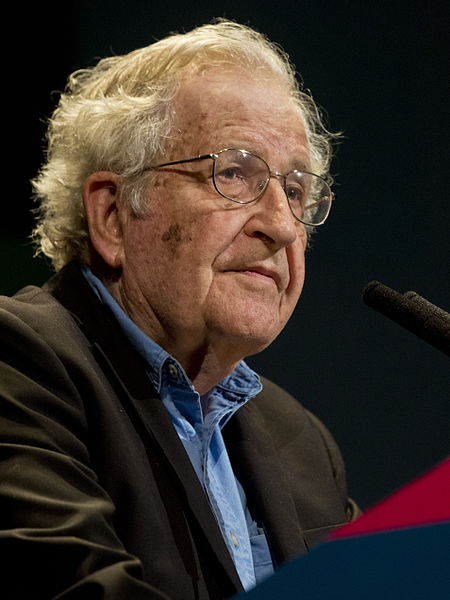
\includegraphics[width=2.5cm]{images/Noam-Chomsky-2015}
% $\;$\rotatebox{90}{\tiny Ministerio de Cultura de la Nación}
% \rotatebox{90}{\tiny 2015, CC-BY-SA 2.0}
% % \bigskip
% 
% "`This world is full of suffering, distress, violence and catastrophes.
% \\Students must decide: does something concern you or not? I say: look around, analyze the problems,
% ask yourself what you can do and set out on the work."' [ZEIT Campus, 2011]
% \end{minipage}\pause
% \hspace{5mm}\ghost{\begin{minipage}{6.0cm}
% 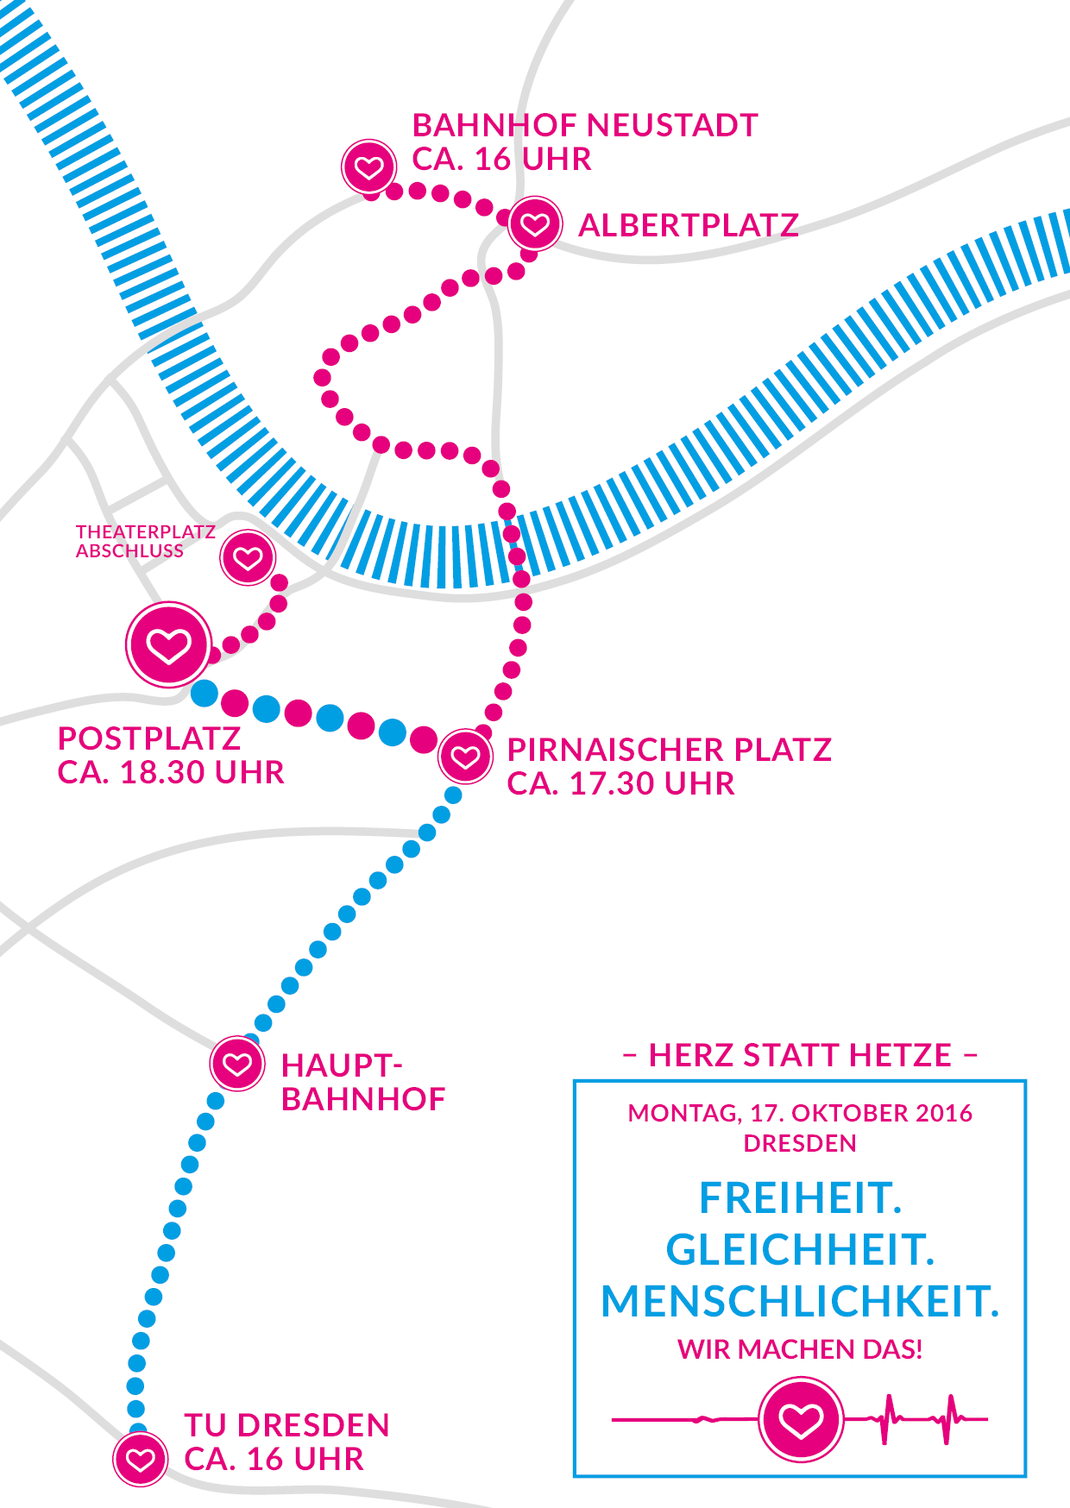
\includegraphics[width=5.9cm]{a2}
% \end{minipage}}\rule[-3cm]{0px}{3px}
% 
% 
% 
% \end{frame}

\begin{frame}\frametitle{Die Chomsky-Hierarchie}

\defbox{
Die \redalert{Chomsky-Hierarchie} unterteilt Grammatiken in vier Stufen:
\begin{itemize}
\item \emph{Typ 0}: beliebige Grammatiken
\item \emph{Typ 1\footnote{Erste Version. Wir werden Typ~1 später noch leicht erweitern.}}: \redalert{kontextsensitive Grammatiken}:\\
	Alle Regeln $w\to v$ erfüllen die Bedingung $|w|\leq|v|$.
\item \emph{Typ 2}: \redalert{kontextfreie Grammatiken}:\\
	Alle Regeln haben die Form $\Snterm{A}\to v$ für eine Variable $\Snterm{A}$.
\item \emph{Typ 3}: \redalert{reguläre Grammatiken}:\\
	Alle Regeln haben eine der Formen
	\[ \Snterm{A}\to \Sterm{c}\Snterm{B}\qquad \Snterm{A}\to \Sterm{c} \qquad \Snterm{A}\to \epsilon\]
	wobei $\Snterm{A}$ und $\Snterm{B}$ Variablen sind und $\Sterm{c}$ ein Terminalsymbol ist.
\end{itemize}

}
\end{frame}

\begin{frame}\frametitle{Chomsky-Hierarchie: Beispiele}

\examplebox{Beispiel: Eine Typ-3-Grammatik (regulär):\\[1ex]
%
\narrowcentering{$\Snterm{S}\to \Sterm{b}\Snterm{A}$
	\hfill $\Snterm{A}\to \Sterm{z}\Snterm{A}$
	\hfill $\Snterm{A}\to \Sterm{z}$}
}\pause

\examplebox{Beispiel: Eine Typ-2-Grammatik (kontextfrei, nicht regulär):\\[1ex]
%
\narrowcentering{$\Snterm{S}\to \Sterm{b}\Snterm{B}\Sterm{z}$
	\hfill $\Snterm{B}\to \Snterm{B}\Sterm{z}\Snterm{B}$
	\hfill $\Snterm{B}\to \epsilon$}
}\pause

\examplebox{Beispiel: Eine Typ-1-Grammatik (kontextsensitiv, nicht kontextfrei):\\[1ex]
%
\narrowcentering{$\Snterm{S}\to \Sterm{b}\Snterm{C}$
	\hfill $\Sterm{b}\Snterm{C}\to \Snterm{S}\Sterm{z}$
	\hfill $\Snterm{S}\Sterm{z}\to \Sterm{bz}$}
}\pause

\examplebox{Beispiel: Eine Typ-0-Grammatik (nicht kontextsensitiv):\\[1ex]
%
\narrowcentering{$\Snterm{S}\to \Sterm{bz}\Snterm{D}\Sterm{z}\Snterm{D}\Sterm{z}$
	\hfill $\Sterm{z}\Snterm{D}\to \Sterm{zz}\Snterm{D}$
	\hfill $\Sterm{z}\Sterm{z}\Sterm{z}\Snterm{D}\Sterm{z}\to \Sterm{z}$}
}
\pause
\smallskip

Alle vier Grammatiken erzeugen die gleiche Sprache $\{\Sterm{b}\}\circ\{\Sterm{z}\}^+$.

\end{frame}

\begin{frame}\frametitle{Kontextfrei und kontextsensitiv}

Der Namensgebung liegt die folgende Idee zugrunde:\medskip

\anybox{gray}{
Typische kontextsensitive Regel:\\[1ex]
\narrowcentering{$\Sterm{a}\Snterm{B}\Sterm{c} \to \Sterm{a}v\Sterm{c} $}\\[1ex]
"`$\Snterm{B}$ kann im Kontext von $\Sterm{a}$ und $\Sterm{c}$ durch $v$ ersetzt werden."'
}
\medskip

\anybox{gray}{
Typische kontextfreie Regel:\\[1ex]
\narrowcentering{$\Snterm{B} \to v $}\\[1ex]
"`$\Snterm{B}$ kann in jedem Kontext durch $v$ ersetzt werden."'
}
\medskip

Allerdings können kontextsensitive Regeln auch andere Formen haben.

\end{frame}

\begin{frame}\frametitle{Typen von Sprachen}

Die Chomsky-Hierarchie kann auf Sprachen angewendet werden:\medskip

\defbox{
Eine Sprache $\Slang{L}$ ist \redalert{vom Typ $i$} wenn sie durch eine Grammatik $G$ von Typ $i$ beschrieben wird, d.h. wenn $\Slang{L}(G)=\Slang{L}$.
Es gibt demnach \redalert{reguläre}, \redalert{kontextfreie} und \redalert{kontextsensitive}
Sprachen.
}
\medskip

Die Beispiele haben gezeigt: man kann die gleiche Sprache oft mit Grammatiken verschiedenen Typs beschreiben.
\medskip

Aber wir werden sehen: für viele Sprachen gibt es einen maximalen Typ von Grammatik, z.B. gibt es kontextfreie Sprachen, die nicht regulär sind.

\end{frame}


\begin{frame}\frametitle{Beziehungen zwischen Chomskys Typen}

Bilden die Typen wirklich eine Hierarchie\\[1ex]
\narrowcentering{"`Typ 3${}\subseteq{}$Typ 2${}\subseteq{}$Typ 1${}\subseteq{}$Typ 0"'?}

\begin{itemize}
\item Jede Grammatik von Typ 1, 2 oder 3 ist auch von Typ 0 (per Definition)
\item Jede reguläre Grammatik ist kontextfrei
(die Typ-3-Regeln
$\Snterm{A}\to \Sterm{c}\Snterm{B}$, $\Snterm{A}\to \Sterm{c}$ und $\Snterm{A}\to \epsilon$ sind auch von Typ 2)
\item Aber nicht jede kontextfreie Grammatik ist kontextsensitiv
(Regeln der Form $\Snterm{A}\to \epsilon$ sind nicht erlaubt)
\end{itemize}

Allgemein können Typ-1-Sprachen in unserer Definition nie das leere Wort enthalten!

\end{frame}


\begin{frame}\frametitle{Typ 1 mit $\epsilon$-Regeln}

Wir erweitern unsere Definition wie folgt:
\defbox{Eine Grammatik $G=\tuple{V,\Sigma,P,S}$ ist von Typ 1 (kontextsensitiv), wenn eine der folgenden Bedingungen gilt:
\begin{enumerate}[(1)]
\item Alle Regeln $w\to v$ erfüllen die Bedingung $|w|\leq|v|$ (ursprüngliche Definition)
%
\item Es gibt eine Regel $S\to\epsilon$ und alle anderen Regeln $w\to v$ erfüllen
	zwei Bedingungen:
	\begin{enumerate}[(a)]
	\item $|w|\leq|v|$ (insbesondere ist also $v\neq\epsilon$)
	\item $S$ kommt nicht in $v$ vor
	\end{enumerate}
	(Sonderfall mit $\epsilon$-Regeln)
\end{enumerate}
}

\examplebox{Beispiel: Die reguläre Grammatik $G$ mit den Regeln\\[1ex]
\narrowcentering{$\Snterm{S}\to \epsilon \mid \Snterm{A}$
	\hfill $\Snterm{A}\to \Sterm{nyan}\Snterm{A}$
	\hfill $\Snterm{A}\to \Sterm{nyan}$}\\[1ex]
ist kontextsensitiv nach der erweiterten Definition. $\Slang{L}(G)=\{\Sterm{nyan}\}^*$.
}

% Die Erweiterung ändert nicht viel:
% \theobox{Eine Sprache $\Slang{L}$ ist kontextfrei nach der erweiterten Typ-1-Definition genau dann wenn
% sie entweder kontext}

\end{frame}

\begin{frame}\frametitle{Kontextfrei vs. kontextsensitiv mit $\epsilon$}

Manche Typ-2-Grammatiken sind weiterhin nicht von Typ 1:
\examplebox{Beispiel: Die kontextfreie (und reguläre) Grammatik\\[1ex]
\narrowcentering{$\Snterm{S}\to \Sterm{b}\Snterm{A}$
	\hfill $\Snterm{A}\to \Sterm{z}\Snterm{A}$
	\hfill $\Snterm{A}\to \epsilon$}
\\[1ex]
ist nicht kontextsensitiv, nicht einmal mit $\epsilon$-Erweiterung.
}

\medskip\pause

\defbox{ Eine kontextfreie Grammatik $G=\tuple{V,\Sigma,P,S}$ ist \redalert{$\epsilon$-frei},
wenn eine der folgenden Bedingungen gilt:
\begin{enumerate}[(1)]
\item Es gibt keine Regel der Form $\Snterm{A}\to\epsilon$
%
\item Es gibt eine Regel $S\to\epsilon$ und bei allen anderen Regeln $\Snterm{A}\to v$
ist $v\neq \epsilon$ und $S$ kommt nicht in $v$ vor.
\end{enumerate}
}

\emph{Offensichtlich:} jede $\epsilon$-freie kontextfreie Grammatik ist \ghost{kontextsensitiv}

\emph{Weniger offensichtlich:} $\epsilon$-freie kontextfreie Grammatiken \ghost{erzeugen}\\ die gleichen Sprachen wie kontextfreie Grammatiken allgemein

% Trotzdem behaupten wir:
% \theobox{
% Jede kontextfreie Sprache ist kontextsensitiv.
% }
% 
% Idee: man kann die problematischen Typ-2-Grammatiken so umformen, dass
% sie von Typ 1 mit $\epsilon$-Regeln sind.

\end{frame}

\begin{frame}\frametitle{Erzeugung $\epsilon$-freier Grammatiken}

Der folgende Algorithmus kann $\epsilon$-Regeln eliminieren.

\codebox{
Eingabe: kontextfreie Grammatik (\redalert{CFG}) $G=\tuple{V,\Sigma,P,S}$\\
Ausgabe: $\epsilon$-freie CFG $G'=\tuple{V',\Sigma,P',S'}$ mit $\Slang{L}(G')=\Slang{L}(G)$
% \medskip
% 
\begin{itemize}
\item Initialisiere $P' \defeq P$ und $V'\defeq V$
% 
\item Berechne $V_\epsilon = \{\Snterm{A}\in V\mid \Snterm{A}\Rightarrow^* \epsilon\}$ \textcolor{devilscss}{(Details dazu später)}
% 
\item Entferne alle $\epsilon$-Regeln aus $P'$
% 
\item Solange es in $P'$ eine Regel $\Snterm{B}\to x\Snterm{A}y$ gibt, mit\\[1ex]
%
\narrowcentering{ $\Snterm{A}\in V_\epsilon$\hfill $|x|+|y|\geq 1$\hfill $\Snterm{B}\to xy\notin P'$ }\\[1ex]
%
wähle eine solche Regel und setze $P'\defeq P'\cup \{\Snterm{B}\to xy\}$
%
\item Falls $S\in V_\epsilon$ dann definiere ein neues Startsymbol $S'\notin V$, setze $V'\defeq V'\cup\{S'\}$ und 
$P'\defeq P'\cup\{S'\to S,S'\to\epsilon\}$.
% 
% 
% füge die Regeln
% %
% \narrowcentering{ $S'\to S$\hfill $S'\to\epsilon$ }\\[1ex]
% %
% in $P'$ ein. 
Falls $S\notin V_\epsilon$, dann verwenden wir einfach $S'\defeq S$ als Startsymbol.
\end{itemize}
}
{\footnotesize (\redalert{CFG} steht für \redalert{context-free grammar} und wird oft als Abkürzung \ghost{verwendet)}}

\end{frame}

\begin{frame}\frametitle{Berechnung von $V_\epsilon$}

Die Variablen $\Snterm{A}\in V$ mit $\Snterm{A}\Rightarrow^* \epsilon$ kann man leicht rekursiv finden:\medskip

\codebox{
Eingabe: kontextfreie Grammatik $G=\tuple{V,\Sigma,P,S}$\\
Ausgabe: $V_\epsilon$ für diese Grammatik
\begin{itemize}
\item Intialisiere $V_\epsilon\defeq \{ \Snterm{A}\mid \Snterm{A}\to\epsilon \in P\}$
\item Solange es eine Regel $\Snterm{B}\to \Sntermsub{A}{1}\ldots \Sntermsub{A}{n}\in P$ gibt, so dass gilt\\[1ex]
%
\narrowcentering{ $\Snterm{B}\notin V_\epsilon$\hfill und \hfill $\Sntermsub{A}{i}\in V_\epsilon$ für alle $i\in\{1,\ldots,n\}$ }\\[1ex]
%
wähle eine solche Regel und setze $V_\epsilon\defeq V_\epsilon\cup \{\Snterm{B}\}$.
\end{itemize}
}\pause

\examplebox{Beispiel:
\begin{minipage}[t]{8cm}
\narrowcentering{%
	$\Snterm{S}\to \Sterm{a}\Snterm{B}\mid \Snterm{BAA}$\hfill
	$\Snterm{B}\to \Sterm{a}\mid \Snterm{AC}$\hfill
	$\Snterm{A}\to \Sterm{bb} \mid \epsilon$}\\[0.5ex]
\narrowcentering{%
	$\Snterm{C}\to \Snterm{DS} \mid \epsilon$\hfill
	$\Snterm{D}\to \Sterm{a}\Snterm{AS}$
}\end{minipage}\\[1ex]
Initialisierung: $V_\epsilon= \{\Snterm{A},\Snterm{C}\}$\\
Schritt 1: $V_\epsilon= \{\Snterm{A},\Snterm{C},\Snterm{B}\}$\\
Schritt 2: $V_\epsilon= \{\Snterm{A},\Snterm{C},\Snterm{B},\Snterm{S}\}$ -- Terminierung
}


\end{frame}

\begin{frame}\frametitle{Beispiel: Eliminierung von $\epsilon$-Regeln}

\examplebox{
\narrowcentering{$\Snterm{S}\to \Sterm{b}\Snterm{B}\Sterm{z}$
	\hfill $\Snterm{B}\to \Snterm{B}\Sterm{z}\Snterm{B}$
	\hfill $\Snterm{B}\to \epsilon$}
}\bigskip\pause

$V_\epsilon= \{\Snterm{B}\}$\medskip\pause

\ghost{\hspace{3.6cm}\begin{minipage}{6cm}
\codebox{
\begin{itemize}
\item Initialisiere $P' \defeq P$
% 
\item Entferne alle $\epsilon$-Regeln aus $P'$
\item Solange es in $P'$ eine Regel $\Snterm{B}\to x\Snterm{A}y$ gibt, mit\\[1ex]
%
\narrowcentering{ $\Snterm{A}\in V_\epsilon$\hfill\hfill $|x|+|y|\geq 1$\hfill\hfill $\Snterm{B}\to xy\notin P'$ }\\[1ex]
%
wähle eine solche Regel und setze $P'\defeq P'\cup \{\Snterm{B}\to xy\}$
\end{itemize}}
\end{minipage}}%
\begin{minipage}[b]{3cm}%
$
\begin{array}{@{}rl}
P' = \pause\{ & \Snterm{S}\to \Sterm{b}\Snterm{B}\Sterm{z},\\
		& \Snterm{B}\to \Snterm{B}\Sterm{z}\Snterm{B},\\
		& \ghost{$\Snterm{B}\to \epsilon,$}\pause\hspace{-2mm}\rotatebox{5}{\rule[0.3ex]{13mm}{1pt}}\\\pause
		& \Snterm{S}\to \Sterm{b}\Sterm{z},\\\pause
		& \Snterm{B}\to \Snterm{B}\Sterm{z},\\\pause
		& \Snterm{B}\to \Sterm{z}\Snterm{B},\\\pause
		& \Snterm{B}\to \Sterm{z} \hspace{5mm}\}\\
\end{array}
$
\end{minipage}

\end{frame}

\begin{frame}\frametitle{Zusammenfassung der Ergebnisse}

Wir können jede CFG in eine $\epsilon$-freie CFG umschreiben. Daher gilt:

\theobox{Satz: Jede kontextfreie Sprache ist kontextsensitiv im erweiterten Sinn (mit $\epsilon$-Sonderfall).}
% \smallskip

Damit gelten alle Inklusionen der Hierarchie. Grafisch dargestellt:\bigskip

\begin{tikzpicture}[decoration=penciline, decorate]
\node (nl) [decorate,draw=nightblue, text depth = 4cm, text width = \linewidth, fill=nightblue!10,thick,align=left, inner ysep=2mm, inner xsep=2mm] at (0,0) {Formale Sprachen};
\node (n0) [decorate,draw=darkgreen, text depth = 3cm, text width = 8cm, fill=darkgreen!10,thick,align=left, inner ysep=2mm, inner xsep=2mm] at ([yshift=-0.5em]nl.center) {Typ-0-Sprachen};
\node (n1) [decorate,draw=strongyellow, text depth = 2cm, text width = 6.7cm,  fill=strongyellow!10,thick,align=left, inner ysep=2mm, inner xsep=2mm] at ([yshift=-0.5em]n0.center) {Kontextsensitive Sprachen (Typ 1)};
\node (n2) [decorate,draw=orange, text depth = 1cm, text width = 5.4cm,  fill=orange!10,thick,align=left, inner ysep=2mm, inner xsep=2mm] at ([yshift=-0.5em]n1.center) {Kontextfreie Sprachen (Typ 2)};
\node (n3) [decorate,draw=red, fill=red!10,thick,align=left, inner ysep=2mm, inner xsep=2mm] at ([yshift=-0.5em]n2.center) {Reguläre Sprachen (Typ 3)};
\end{tikzpicture}

\end{frame}

\begin{frame}\frametitle{Zusammenfassung und Ausblick}

Nicht alle Sprachen sind mathematisch beschreibbar oder durch Computer entscheidbar
\bigskip

\redalert{Induktion} (= rekursive Konstruktion von Beweisen) ist oft nötig, um Behauptungen
über unendliche Sprachen zu beweisen
\bigskip

\redalert{Grammatiken} können (manche) Sprachen beschreiben. Die \redalert{Chomsky-Hierarchie} teilt Grammatiken 
in vier Typen ein.
\bigskip

\anybox{yellow}{
Offene Fragen:
\begin{itemize}
\item Was gewinnt man durch die Beschränkung auf spezielle Typen?
\item Sind die Typen wirklich unterschiedlich?
\item Wie kommt Berechnung ins Spiel?
\end{itemize}
}

\end{frame}


\end{document}
